\documentclass[]{article}
\usepackage{amsmath}\usepackage{amsfonts}
\usepackage[margin=1in,footskip=0.25in]{geometry}
\usepackage{mathtools}
\usepackage{hyperref}
\hypersetup{
    colorlinks=true,
    linkcolor=blue,
    filecolor=magenta,
    urlcolor=cyan,
}
\usepackage[final]{graphicx}
\usepackage{listings}
\usepackage{courier}
\lstset{basicstyle=\footnotesize\ttfamily,breaklines=true}
\newcommand{\indep}{\perp \!\!\! \perp}
% \usepackage{wrapfig}
\graphicspath{{.}}

\begin{document}

Name: Hongda Li
\par
Class: AMATH 585 2022 WINTER HW2
\section*{Problem 1}
    \subsection*{1(a)}
        Let $c(x)$ be the thermal conductivity function, and we can continue from the results in (2.73). We assume equally spaced grid points with $x_1, x_2, \cdots x_m$ denoting the interior points and $x_{m + 1}, x_0$ denotes the right and left boundary points. For the interior points, the system is denoted as: 
        \begin{align*}\tag{1.a.1}\label{eqn:1.a.1}
            \frac{1}{h^2}(
                    c_{i + 1/2}u_{i + 1} 
                    - (c_{i - 1/2} + c_{i + 1/2})u_i +
                    c_{i - 1/2}u_{i - 1}
                ) = f(x_i)\quad \forall \; 2 \le i \le m
        \end{align*}
        Here, $c_i = c(x_i)$ and $x_i = ih$. \\
        Then for the boundary points, we are going to use the $u(0) = 1$ to modify the case where $i = 1$, and then we will roll back the right boundary points, using a first order central difference scheme. 
        \begin{align*}\tag{1.a.2}\label{eqn:1.a.2}
            \frac{1}{h^2}(
                c_{3/2}u_2 - (c_{1/2} + c_{3/2})u_1 + c_{1/2}u_0
            ) &= f(x_1)
            \\
            \text{let: }u_0 &= 1
            \\
            \frac{1}{h^2}(c_{3/2}u_2 - (c_{1/2} + c_{3/2})u_1)
            &= 
            f(x_1) - \frac{f(x_{1/2})}{h^2}
        \end{align*}
        And for the Neuman boundary condition we can roll it back like: 
        \begin{align*}\tag{1.a.3}\label{eqn:1.a.3}
            \frac{1}{2h}(3u_{m + 1} - u_m + u_{m + 1}) &= 0
            \\
            3u_{m + 1} - 4u_m + u_{m - 1} &= 0
            \\
            3u_{m + 1} &= 4u_m - u_{m - 1}
            \\
            u_{m + 1} &+ \frac{1}{3}(4u_m - u_{m - 1})
        \end{align*}
        Consider the last row of \hyperref[eqn:1.a.1]{1.a.1} with $i = m$: 

        \begin{align*}\tag{1.a.4}\label{eqn:1.a.4}
            \frac{1}{h^2}\left(
                    c_{m + 1/2}u_{m + 1}
                    -
                    (c_{m - 1/2} + c_{m + 1/2})u_m + 
                    c_{m - 1/2}u_{m + 1}
                \right) &= f(x_m)
            \\
            \text{Let: }u_{m + 1} &= \frac{1}{3}(4u_m - u_{m - 1})
            \\
            \frac{1}{h^2}\left(
                \frac{c_{m + 1/2}}{3}(4u_m - u_{m - 1}) - 
                (c_{m - 1/2}+ c_{m + 1/2})u_m + 
                c_{m - 1/2}u_{m - 1}
            \right) &= f(x_m)
            \\
            \frac{1}{h^2}\left(
                \left(
                    \frac{4}{3}c_{m + 1/2} - c_{m - 1/2} - 
                    c_{m + 1/2}
                \right)u_m + 
                \left(
                    c_{m - 1/2} - \frac{c_{m + 1/2}}{3}
                \right)u_{m - 1}
            \right) &= f(x_m)
            \\
            \frac{1}{h^2}\left(
                \left(
                    \frac{1}{3}c_{m + 1/2} - c_{m - 1/2}
                \right)u_m + 
                \left(
                    c_{m - 1/2} - \frac{c_{m + 1/2}}{3}
                \right)u_{m - 1}
            \right) &= f(x_m)
        \end{align*}
    \subsection*{1(b)}
        I just coded it in, and get the following code in julia:
        \begin{verbatim}
# For HW 2. Problem 1 
# similate the non-homogenous heat conductivity problem. 

using SparseArrays

"""
    (c(x)u'(x))' = f(x), with u(0) = 1, u'(1) = 0 
    1d BVP.
    Parameter m: 
        It defines the grids. 
        Grids: x0, x1, ... xm, x(m + 1)
        h: 1/(m + 1)
        u0 = 0, which simplifies the system to a (m + 1)x(m + 1) system. 
        So, m is the number of interior points for the domain of the function. 
    Parameter c: 
        A function for scalar that is the thermal conductivity on the rod. 
    Returns: 
        The matrix A to solve and an additional vector for modifying the 
        RHS, which is the boundary conditions.
"""
function FiniteDiffMatrix(m::Int64, c::Function)
    h = 1/(m + 1)
    dict = Dict{Tuple{Int64, Int64}, Float64}()
    
    # first row
    dict[1, 1] = -(c(3*h/2) + c(h/2))/h^2
    dict[1, 2] = c(3*h/2)/h^2
    for i in 2:m
        dict[i, i - 1] = c((i - 1/2)*h)/h^2
        dict[i, i]     = -(c((i + 1/2)*h) + c((i - 1/2)*h))/h^2
        dict[i, i + 1] = c((i + 1/2)*h)/h^2
    end
    
    # Last row
    dict[m + 1, m]     = (c((m + 3/2)*h) + c((m + 1/2)*h))/h^2
    dict[m + 1, m + 1] = -(c((m + 3/2)*h) + c((m + 1/2)*h))/h^2
    
    # coordinate format. 
    CooFormatx = Vector{Float64}()
    CooFormaty = Vector{Float64}()
    CooFormatval = Vector{Float64}()
    for (K, V) in dict
        push!(CooFormatx, K[1])
        push!(CooFormaty, K[2])
        push!(CooFormatval, V)
    end
    
    # boundary modifications
    b = zeros(m + 1)
    b[1] =  - c(h/2)/h^2
    
    # sparse matrix. 
    return sparse(CooFormatx, CooFormaty, CooFormatval), b
end


"""
    Solve the system: (c(x)u'(x))' = f(x), with u(0) = 1, u'(1) = 0 
    for c(x) = (1 + x)^2. 
"""
function SolveFor(f::Function, m::Int64)
    c(x) = (1 + x^2)
    h = 1/(m + 1)
    A, b = FiniteDiffMatrix(m, c)
    y = f.(LinRange(0, 1, m + 2)[2:end])
    RHS = y + b
    display(A)
    display(RHS)
    u = A\RHS
    return vcat(1, u)
end


# Basic testing
using Plots, LinearAlgebra, Latexify
m = 3
f = (x) -> 2(3x^2 - 2x + 1)
u = SolveFor(f, m)
uhat = (x) -> (1 - x)^2
x = LinRange(0, 1, m + 2)

fig = plot(x, u)
plot!(fig, x, uhat.(x))

# Verify the Errors rate
Errors = Vector{Float64}()
Hs = Vector{Float64}()
for m in 2 .^ collect(1:12) .- 1
    x = LinRange(0, 1, m + 2)
    h = 1/(m + 1)
    u = SolveFor(f, m)
    push!(Errors, sqrt(h)*norm(u - uhat.(x)))
    push!(Hs, h)
end

fig = plot(log2.(Hs), log2.(Errors), title="Error Log2 Log2")
savefig(fig, "errorloglog.png")

display(latexify(hcat(Hs, Errors)))

            
        \end{verbatim}
    \subsection*{1(c)}
        Differet values of $h$ ins investigated, and here is a table of errors and corresponding h. 
        \begin{equation}\tag{1.c.1}\label{eqn:1.c.1}
            \begin{array}{|c|c|}
                \text{h}  & \Vert e\Vert_{L2}\\
                0.5 & 0.044501963163344684 \\
                0.25 & 0.011187854310463333 \\
                0.125 & 0.0027213761549214383 \\
                0.0625 & 0.0006665339286528997 \\
                0.03125 & 0.0001646589453009265 \\
                0.015625 & 4.0903149563366545e-5 \\
                0.0078125 & 1.0192189097546314e-5 \\
                0.00390625 & 2.5437920722410657e-6 \\
                0.001953125 & 6.354128827023392e-7 \\
                0.0009765625 & 1.587869820774079e-7 \\
                0.00048828125 & 3.969310322868865e-8 \\
                0.000244140625 & 9.940604664997173e-9 \\
                \end{array}
        \end{equation}

    And here is a loglog plot of the $h$ step sizes against the Error measured under 2 norm: 
    \begin{center}
        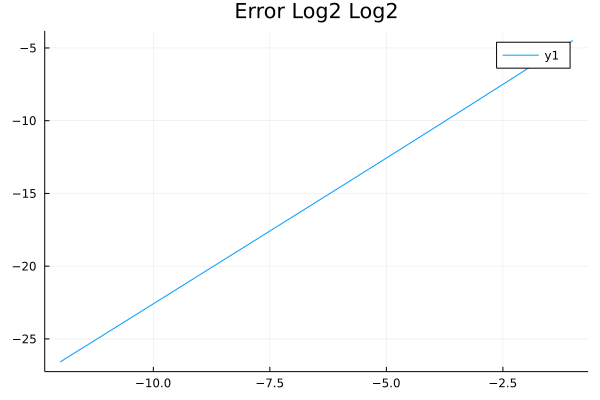
\includegraphics[width=10cm]{errorloglog.png}    
    \end{center}
    

\section*{Problem 2}
    \subsection*{2(a)}
        The system is: 
        \begin{align*}\tag{2.a.1}\label{eqn:2.a.1}
            \begin{bmatrix}
                1/9 & & & \\
                1 & - 2 & 1 & \\
                & 1 & -2 & 1 \\ 
                & & & 1/9
            \end{bmatrix}
            \begin{bmatrix}
                u_0 \\ u_1 \\ u_2 \\ u_4
            \end{bmatrix}
            &= 
            \begin{bmatrix}
                1 \\ f(x_1) \\ f(x_2) \\ 1
            \end{bmatrix}
        \end{align*}

    \subsection*{2(b)}
        If $B$ is the inverse of $A$, the second and third columns of B are $hG(\vec{x}, x_j)$. The first and second columns are $G_0(\vec{x}), G_1(\vec{x})$. Let the indices for matrix $B$ begins with zero. Then it's given as: 
        \begin{align*}\tag{2.b.1}\label{eqn:2.b.1}
            B_{i, j} &= 
            hG(x_i, x_j) = 
            \begin{cases}
                h(x_j- 1)x_i & i = 1, 2, \cdots j
                \\
                h(x_i - 1)x_j & i = j, j+ 1, \cdots, m
                \\
                0 & i = m + 1, 0
            \end{cases}
            \\
            B_{i, 0} &= G_0(x_i) = 1 - x_i \quad \forall \; 0\le i \le m + 1
            \\
            B_{i, m + 1} &= G_1(x_i) = x_i \quad \forall \;0 \le i \le m + 1
        \end{align*}
        Those are from the lecture.
        \\
        In our case, substituting in $h = 1/3$, we have: 
        \begin{align*}\tag{2.b.2}\label{eqn:2.b.2}
            B&= \begin{bmatrix}
                1 & 0 & 0 & 0 \\
                2/3& (1/3)(-2/3)(1/3) &(1/3)(-1/3)(1/3) & 1/3
                \\
                1/3 & 1/3(-1/3)(1/3) & (1/3)(-1/3)(2/3) & 2/3
                \\
                0 & 0& 0& 1
            \end{bmatrix}
            \\
            &=  
            \begin{bmatrix}
                1 & 0 & 0 & 0 \\
                2/3& -2/27 & -1/27 & 1/3
                \\
                1/3 & -1/27 & -2/27 & 2/3
                \\
                0 & 0& 0& 1
            \end{bmatrix}
        \end{align*}
    \subsection*{2(c)}
    Let the RHS $f(x) = x$, then the scketches for the 4 Greens Function and the solution will be like: 
    % insert scketches of the Greens function and solution here. 
    \begin{center}
        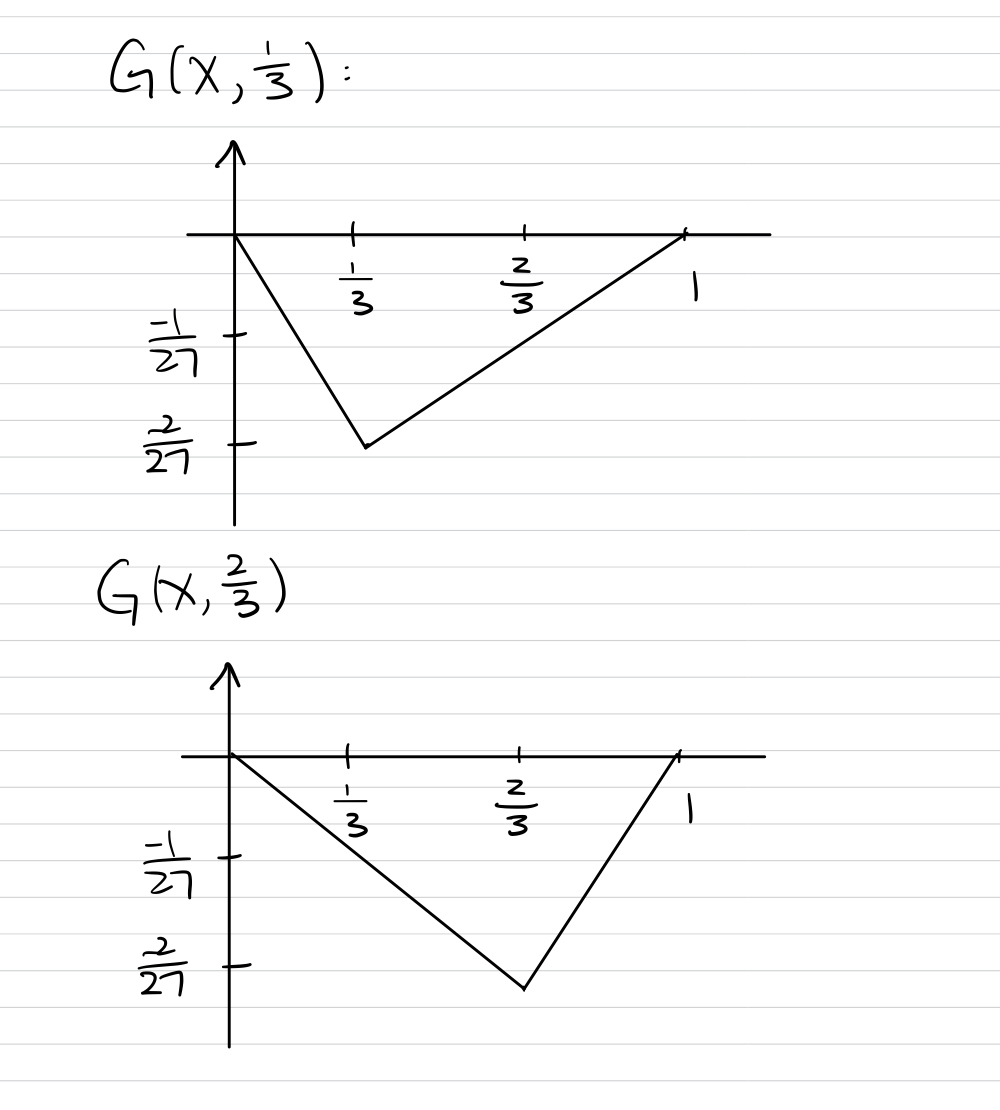
\includegraphics[width=8cm]{green_sketch1.jpeg}
    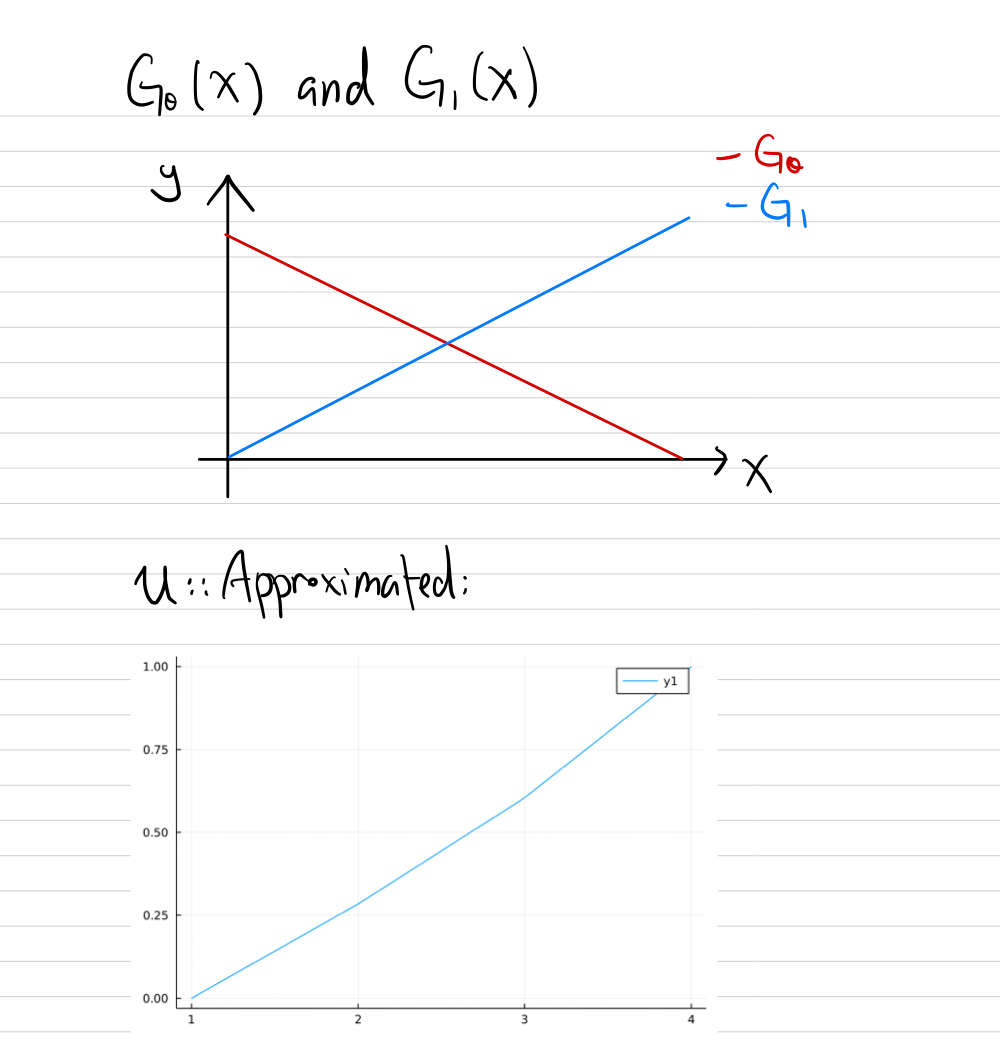
\includegraphics[width=8cm]{green_sketch2.jpeg}    
    \end{center}
    
\section*{Problem 3}
    \subsection*{3(a)}
        Assume that there are $m$ intervals with $m + 1$ grid points with the both boundaries, index starts with zero: $x_0, x_1, \cdots x_m$, equally spaced points with width $h$ over the interval $[a, b]$. 
        \\
        We wish to prove the the trapzoidal rules approximation has an error of $\mathcal{O}(h^2)$ globally. When $g(x)$ is smooth, it has: 
        \begin{align*}\tag{3.a.1}\label{eqn:3.a.1}
            g(x + h) &= g(x) + \frac{h^2}{2}g''(x) + \mathcal{O}(h^3)
        \end{align*}
        Now consider: 
        \begin{align*}\tag{3.a.2}\label{eqn:3.a.2}
            &\hspace{1.1em} 
            \frac{h(g(x_j) + g(x_j + h))}{2}\\
            &= 
            \frac{h}{2}\left(
                2g(x_j) + hg'(x_j) + \frac{h^2}{2}g''(x_j)
                + \mathcal{O}(h^3) 
            \right)
            \\
            &= 
            hg(x_j) + \frac{h}{2}\left(
                hg'(x_j) + \frac{h^2}{2}g''(x_j) + \mathcal{O}(h^3)
            \right)
            \\
            &= 
            hg(x_j) +  \frac{1}{2}\left(
                h^2g'(x_j) + \frac{h^3}{2}g''(x_j) + \mathcal{O}(h^4)
            \right)
        \end{align*}
        This serves as the approximations to the integral of $g(x)$ over the interval $[x_j, x_{j + 1}]$, let's compare it with the integral form: 
        \begin{align*}\tag{3.a.3}\label{eqn:3.a.3}
            & \hspace{1.1em}
            \int_{x_j}^{x_{j + h}} g(x)dx \quad \text{usub}: x = x_j+ \xi\\ 
            &= \int_{0}^{h} 
                g(x_j) + \xi g'(x_i) + \frac{\xi^2}{2}g''(x_j) + 
                \mathcal{O}(\xi^3)
            d\xi
            \\
            &= hg(x_j) + \frac{h^2}{2}g'(x_j) + \frac{h^3}{3!}g''(x_j) + \mathcal{O}(h^4)
        \end{align*}
        Now we can compare the integral and the discretized approximations by taking the differences between them. 
        \begin{align*}\tag{3.a.4}\label{eqn:3.a.4}
            &\hspace{1.1em}
            \int_{x_j}^{x_j + h} 
            g(x)
            dx - \frac{h}{2}\left(
                g(x_j) + g(x_j + h)
            \right)
            \\
            &= 
            hg(x_j) + \frac{h^2}{2}g'(x_j) + \frac{h^3}{3!}g''(x_j) + \mathcal{O}(h^4) - 
            hg(x_j) - 
            \frac{1}{2}
            \left(
                h^2g'(x_j) + \frac{h^3}{2}g''(x_j) + \mathcal{O}(h^4)
            \right)
            \\
            &= \frac{h^3}{3!}g''(x_j) - \frac{h^3}{2}g''(x_j) + \mathcal{O}(h^4)
            \\
            &= \frac{-h^3}{3}g''(x_j) + \mathcal{O}(h^4)
            \\
            &= \mathcal{O}(h^3)
        \end{align*}
        When we add up these local approximations we lose one order of accuracy globally. But before we proceed to prove that, we have to assume that the second derivative of $g(x)$ is bounded by $M$ over the integral $[a, b]$ in term of the absolute value. Then we can consider: 
        \begin{align*}\tag{3.a.5}\label{eqn:3.a.5}
            &\hspace{1.1em}
            \int_{b}^{a}g(x)dx - \sum_{j = 0}^{m}
            \frac{h(g(x_j) - g(x_j + h))}{2}
            \\
            &= \sum_{j = 0}^{m}
            \int_{x_j}^{x_{j + 1}} g(x)dx - 
            \frac{h}{2}(g(x_j)+ g(x_j + h))
            \\
            &= 
            \sum_{j = 0}^{m}\frac{h^3}{3!}g''(x_j) - 
            \frac{h^3}{2}g''(x_j) + \mathcal{O}(h^4)
            \\
            &= \sum_{j = 0}^{m} \frac{-g''(x_j)h^3}{3} + \mathcal{O}(h^4)
            \\
            \left|\sum_{j = 0}^{m} \frac{-g''(x_j)h^3}{3} + \mathcal{O}\right|
            & \le 
            \frac{mMh^3}{3} + \mathcal{O}(h^3)
            \\
            \text{Notice: } m = \frac{b - a}{h} 
            \\
            \frac{mMh^3}{3} + \mathcal{O}(h^3) &= 
            \mathcal{O}(h^2)
        \end{align*}
    Globally the error is $h^2$, if we assume the function has bounded second deriative and it's smooth.
    \subsection*{3(b)}
        We are concerned with the BVP problem: 
        \begin{align*}\tag{3.b.0}\label{eqn:3.b.0}
            \begin{cases}
                u''(x) = f(x) & x\in[0, 1]
                \\
                u(0) = u(1) =0
            \end{cases}
        \end{align*}
        The solution in integral form using Green's Function and the solution in summation form using a summation are here: 
        \begin{align*}\tag{3.b.1}\label{eqn:3.b.1}
            u(x) &= \int_{0}^{1} 
                f(\bar{x})G(x|\bar{x})
            d\bar{x}
        \end{align*}
        \begin{align*}\tag{3.b.2}\label{eqn:3.b.2}
            u_i &= h \sum_{j = 1}^{m}f(x_j)G(x_i|x_j) \quad i = 1\cdots m
        \end{align*}
        We make the same type of assumptions about the grid points as 3(a). And then we wish to show that, expression \hyperref[eqn:3.b.2]{3.b.2} is the trapzoidal approximation to \hyperref[eqn:3.b.1]{3.b.1}. 
        \\
        Consider the quantity $u(x_i)$: 
        \begin{align*}\tag{3.b.3}\label{eqn:3.b.3}
            u(x_i) &= \int_{0}^{1} 
                f(\bar{x})G(x|\bar{x})
            d\bar{x}
            \\
            & \approx
            \sum_{j = 0}^{m}\frac{h}{2}\left(
                f(x_j)G(x_i|x_j) + f(x_{j + 1})G(x_i| x_{j + 1})
            \right)
            \\
            &= 
            \sum_{j=0}^{m}\frac{h}{2}f(x_j)G(x_i|x_j)
            +
            \sum_{j - 1}^{m + 1}\frac{h}{2}f(x_j)G(x_i|x_j)
            \\
            &= \frac{h}{2}(
                f(x_0)G(x_i|x_0) + f(x_{m + 1})G(x_i|x_{m + 1})
            ) + 
            \sum_{j = 1}^{m}hf(x_j)G(x_i|x_j)
            \\
            &= 
            0 + \underbrace{\sum_{j = 1}^{m}hf(x_j)G(x_i|x_j)}_{= u_i}
        \end{align*}
        $G(x_i|x_{m + 1}) = 0$ and $G(x_i|x_0) = 0$ because of the boundary conditions from \hyperref[eqn:3.b.0]{3.b.0}, that is how we got from the second last equality to the last equality above. 
        \\
        Therefore the error between the analytical solution using the integral form and the Green's Function and the discretized linear combinations of the Green's Function (also the solution from the linear system) has an error $\mathcal{O}(h^2)$. 
        \\
        In addition, the discontinuity of the Green's function first derivative and the unbounded second deriative of Greens' Function doesn't impact the accuracy is because the pint of discontinuity is exactly at the grid point $x_j$. And for every $x\in[x_j, x_{j + 1}]$, the integrand $f(\bar{x})G(x|\bar{x})$ is smooth and has bounded second derivative. Hence we can still use the derived $\mathcal{O}(h^2)$ from \hyperref[eqn:3.a.5]{3.a.5}. 
\section*{Problem 4}
    \subsection*{4(a)}
        $G_0(x)$ solves $u''(x) = 0$, with BC: $u'(0) = 1, u(1) = 0$. Which means that: 
        \begin{align*}\tag{4.a.1}\label{eqn:4.a.1}
            \iint u(x)dxdx &=\iint 0 dxdx
            \\
            & = Cx + D 
            \\
            \left.\partial_x(Cx + D)\right|_{x = 0} &= 1
            \\
            \implies C &= 1
            \\
            \left.(Cx + D)\right|_{x =1} &= 0
            \\
            \implies D &= -1 
            \\
            \implies G_0(x) &= x - 1
        \end{align*}
        Next we solve for $G_1(x)$ as the solution to the problem $u''(x) = 0$, $u'(0) = 0$, $u(1) = 1$. Similar to the previous case in (4.a.1), the solution of the Green's Function will atke the form $Cx + D$, and: 
        \begin{align*}\tag{4.a.2}\label{eqn:4.a.2}
            \left.\partial_x (Cx + D)\right| &= 0
            \\
            \implies C &= 0
            \\
            \left. 
                Cx + D     
            \right|_{x = 1} &= 1
            \\
            \implies D &= 1
            \\
            \implies G_1(x) &= 1
        \end{align*}
        Next, we are interested in the Green's Function that Solves the Delta function. We are solving $u''(x) = \delta(x - \bar{x})$, $u'(0) = 0, u(1) = 0$. To solve it we would need 3 sets of properties. $G(x|\bar{x})$ is continuous, there is a unit jump in the derivative from $\bar{x} - \epsilon$ to $\bar{x} + \epsilon$ and it has to satisfies the boundary conditions for the problems. 
        \begin{align*}\tag{4.a.3}\label{eqn:4.a.3}
            &\hspace{1.1em}
            \int_{0}^{\bar{x} - \epsilon} \int_{0}^{\bar{x} - \epsilon} 
            G(x|\bar{x}) dxdx
            \\
            &= C_1x + C_2
            \quad \forall x \in [0, \bar{x} - \epsilon]
            \\
            &\hspace{1.1em} 
            \int_{\bar{x} - \epsilon}^{1}
            \int_{\bar{x} - \epsilon}^1
            G(x|\bar{x})dxdx 
            \\
            &= C_3x + C_4
            \quad \forall x \in [\bar{x} + \epsilon, 1]
            \\
            \implies G(x|\bar{x}) &=
            \begin{cases}
                C_1x + C_2 & x\in [0, \bar{x}]
                \\
                C_3x + C_4 & x \in [\bar{x}, 1]
            \end{cases}
        \end{align*}
        Next we solev for these coefficients (We assume that $\bar{x} \in (0, 1)$): 
        \begin{align*}\tag{4.a.4}\label{eqn:4.a.4}
            G'(0|\bar{x}) \implies \partial_x \left.[C_1x + C_2]\right|_{x = 0} &= 
            0
            \\ \implies 
            C_1 &= 0 
            \\
            G(1|\bar{x}) =0 \implies C_3 + C_4 &= 0 \implies C_4 = -C_3
            \\
            \implies 
            G(x|\bar{x}) &= \begin{cases}
                C_2 & x \in [0, \bar{x}]    
                \\
                C_3x - C_3 & x\in [\bar{x}, 1]
            \end{cases}
            \\
            \lim_{\epsilon \searrow 0}
            G'(\bar{x} + \epsilon| \bar{x}) - G'(\bar{x} - \epsilon|\bar{x}) &= 1
            \\
            \implies C_3 - 0 &= 1 \implies C_3 = 1
            \\
            \implies 
            G(x|\bar{x}) &= \begin{cases}
                C_2 & x \in [0, \bar{x}]    
                \\
                x - 1 & x\in [\bar{x}, 1]
            \end{cases}
        \end{align*}
        Finally, we knwo that the function $G(x|\bar{x})$ is continuous on the point $\bar{x}$, which means that $C_2 = \bar{x} - 1$, therefore we have the final representation for the Green's Function as: 
        \begin{align*}\tag{4.a.5}\label{eqn:4.a.5}
            G(x|\bar{x}) &= \begin{cases}
                \bar{x} - 1 & x \in [0, \bar{x}] 
                \\
                x - 1 & x \in [\bar{x}, 1]
            \end{cases}
        \end{align*}
        So the left side of the Delta RHS Green's Function has a negative constant on the interval $[0, \bar{x}]$, and it's increasing on interval $[\bar{x}, 1]$ with a slope of 1. 
        \\
        Next, we are combinging the Green's Function and use it to get the columns of the $A^{-1}$. From \hyperref[eqn:3.b.3]{3.b.3}, we know that the solution is a linear combinations of the function $G(\vec{x}|x_j)$ for the $j^{th}$, intuitively, the solution can be viewed as a linear combinations of the columns of the discretized operator. Here, it's not hard to see that the solution of the mixed boundary conditions listed above \hyperref[eqn:4.a.1]{4.a.1} can be written as: 
        \begin{align*}\tag{5.a.6}\label{eqn:5.a.6}
            \vec{u} &= \alpha G_0(\vec{x}) + \sum_{j= 1}^{m}
            hf(\vec{x})G(\vec{x}| x_j) + \beta G_1(\vec{x})
        \end{align*}
        This will be useful for the next part of the question. 
    \subsection*{4(b)}
        Here is the discretized system given from (2.54), and we are intersted in looking for the inverse of the matrix $A$: 
        \begin{align*}\tag{4.b.1}\label{eqn:4.b.1}
            Au &= f 
            \\
            \frac{1}{h^2} \begin{bmatrix}
                -h & h  & & & &\\
                1 & -2 & 1 & & & \\
                & 1 & -2 & 1 & &  \\[0.2em] 
                & & \ddots & \ddots & \ddots & \\
                & & & 1& -2&1\\
                & & & & 0 & h^2 
            \end{bmatrix}
            \begin{bmatrix}
                u_0 \\ u_1 \\ \vdots \\ v_{m - 1} \\ v_{m} \\ v_{m + 1}
            \end{bmatrix} &= 
            \begin{bmatrix}
                \delta \\f(x_1) \\f(x_2)\\\cdots \\f(x_{m - 1}) \\f(x_m)
                \\ 
                \beta
            \end{bmatrix}
        \end{align*}
        Similar to the example where we did in class, the columns of $A^{-1}$ are the Green's Function we solved in part 4(a), and the intuitive understanding are discussed in \hyperref[eqn:5.a.6]{5.a.6}. Therfore the claim I make is: 
        \begin{align*}\tag{4.b.2}\label{eqn:4.b.2}
            (A^{-1})_{:, 1} &= G_0(\vec{x}) 
            \\
            (A^{-1})_{:, m + 1} &= G_2(\vec{x}) 
            \\
            (A^{-1})_{:, j} &= hG_2(\vec{x}) 
        \end{align*}
        Take this for granted, and I also didn't put $h$ for the boundary Green's Function. Let's consider the specific case where $h = 1/3$ so that $A$ would be a 4 by 4 matrix, and the inverse we wish to find will be 4 by 4. Recall the Greens function we figured out in \hyperref[eqn:4.a.1]{4.a.1}, \hyperref[eqn:4.a.2]{4.a.2}, and \hyperref[eqn:4.a.5]{4.a.5}. Then $A^{-1}$ is like: 
        \begin{align*}\tag{4.b.3}\label{eqn:4.b.3}
            (A^{-1})_{:, 0} &= \begin{bmatrix}
                0 \\1/3 \\2/3\\ 1
            \end{bmatrix}
            - \begin{bmatrix}
                1 \\1 \\1\\ 1 
            \end{bmatrix}
            = 
            \begin{bmatrix}
                -1\\ -2/3\\ -1/3\\ 0
            \end{bmatrix}
            \\
            (A^{-1})_{:, 3} &= 
            \begin{bmatrix}
                1 \\ 1 \\ 1 \\ 1
            \end{bmatrix}
        \end{align*}
        Using the Interior Green's Function from \hyperref[eqn:4.a.5]{4.a.5}. 
        \begin{align*}\tag{4.b.4}\label{eqn:4.b.4}
            (A^{-1})_{:, 1} &= \frac{1}{3}
            G\left(\vec{x}\left|\frac{1}{3}\right.\right)
            \\
            &= \frac{1}{3}
            \begin{bmatrix}
                -2/3 \\ -2/3 \\ -1/3 \\ 0
            \end{bmatrix}
            \\
            (A^{-1})_{:, 2} &= \frac{1}{3}
            G\left(\vec{x}\left|\frac{2}{3}\right.\right)
            \\
            &= \frac{1}{3}\begin{bmatrix}
                -1/3\\ -1/3\\ -1/3\\ 0
            \end{bmatrix}
            \\
            \implies A^{-1} &= 
            \begin{bmatrix}
                -1 & -2/9 & -1/9 & 1\\
                -2/3 & -2/9 & -1/9 & 1\\ 
                -1/3 & -1/9& -1/9 & 1\\
                0 & 0 & 0 & 1
            \end{bmatrix}
        \end{align*}
    \subsection*{5}
        We wish to find the null space of $A^T$. To establish the problem we introduce in (2.58) back in the textbook. To consider the matrix differently, I will represent the matrix as a block 3 by 3 matrix: 
        \begin{align*}\tag{5.1}\label{eqn:5.1}
            A &= \frac{1}{h^2} 
            \begin{bmatrix}
                -h & h(\mathbf{e}^{(m)}_1)^T & 0 \\
                \mathbf{e}_1^{(m)} & \tilde{A} & \mathbf{e}^{(m)}_m \\ 
                0 & h(\mathbf{e}_m^{(m)}) & - h
            \end{bmatrix} 
            \quad
            \text{Where } 
            \tilde{A} = \begin{bmatrix}
                -2 & 1  & & &  \\
                1 & -2 & 1 & &  \\
                & &\ddots &\ddots &  \\ 
                & & & & 1  \\ 
                & & &1 & -2 \\ 
            \end{bmatrix}
        \end{align*}
        And from lecture we know that $\tilde{A}$ is invertible. Next, we find the $A^T$ and the solve the system $Ay = \mathbf{0}$. We introduce the notation of $\mathbf{e}_i^{m}$ denoting the $i$ standard basis vector in $\mathbb{R}$. 
        \begin{align*}\tag{5.2}\label{eqn:5.2}
            A^T &= 
            \frac{1}{h^2}\begin{bmatrix}
                -h & (\mathbf{e}^{(m)}_1)^T & 0 \\
                h\mathbf{e}_1^{(m)} & \tilde{A} & h\mathbf{e}^{(m)}_m \\ 
                0 & (\mathbf{e}_m^{(m)})^T & - h
            \end{bmatrix} 
            \\
            \frac{1}{h^2}\begin{bmatrix}
                -h & (\mathbf{e}^{(m)}_1)^T & 0 \\
                h\mathbf{e}_1^{(m)} & \tilde{A} & h\mathbf{e}^{(m)}_m \\ 
                0 & (\mathbf{e}_m^{(m)})^T & - h
            \end{bmatrix} 
            \begin{bmatrix}
                x_1 \\ y \\ x_2
            \end{bmatrix}
            & =
            \begin{bmatrix}
                0 \\ \mathbf{0} \\ 0
            \end{bmatrix}
            \\
            \begin{bmatrix}
                -hx_1 + y_1 
                \\
                hx_1 \mathbf{e}_1^{(m)} + \tilde{A}y + hx_2 \mathbf{e}_m^{(m)}
                \\
                y_m -x_2 h
            \end{bmatrix}
            & =
            \begin{bmatrix}
                0 \\ \mathbf{0} \\ 0
            \end{bmatrix}
            \\
            \implies & 
            \begin{cases}
                y_1 = hx_1 \\ 
                y_m = hx_2
            \end{cases}
        \end{align*}
        Let's focus on the middle row of the system of equation, and substitute $hx_1, hx_2$ with $y_1, y_m$ then it's giving us: 
        \begin{align*}\tag{5.3}\label{eqn:5.3}
            y_1 \mathbf{e}_1^{(m)} + \tilde{A}y + y_m \mathbf{e}_m^{(m)} 
            &= \mathbf{0}
            \\
            (\tilde{A} + \mathbf{e}^{(m)}_1\mathbf{e}^{(m)T}_1 + \mathbf{e}_m^{(m)}\mathbf{e}_m^{(m)T}) y &= \mathbf{0}
            \\
            \begin{bmatrix}
                -1 & 1 & & \\
                1 & -2 & 1 & \\
                & 1& -2& 1 \\
                & & & \ddots & \\
                & & & -1&1 
            \end{bmatrix} y = \mathbf{0}
            \\
            \implies
            y \in \text{span}\left(
                \begin{bmatrix}
                    1 \\ \vdots \\ 1
                \end{bmatrix}
            \right)P
        \end{align*}
        And therefore, it's not hard to see that $x_1 = 1/h$ and $x_2 = 1/h$ as well. And hence the null space of the matrix $A$ would be given by: 
        $$
            \text{null}(A^T) = \text{span}\left(
                \begin{bmatrix}
                    1/h \\ 1 \\ \vdots \\ 1 \\ 1/h
                \end{bmatrix}
            \right)ns
        $$
\section*{Problem 6}
    \subsection*{6(a)}
        Consider the discretized system $Au =f$ given as: 
        $$
            \frac{1}{h^{2}}\left(\begin{array}{ccccc}
            -h & h & & & \\
            1 & -2 & 1 & & \\
            & 1 & \ddots & \ddots & \\
            & & \ddots & \ddots & 1 \\
            & & & 1 & -2
            \end{array}\right)\left(\begin{array}{c}
            u_{0} \\
            u_{1} \\
            \vdots \\
            u_{m-1} \\
            u_{m}
            \end{array}\right)=\left(\begin{array}{c}
            \sigma+(h / 2) f\left(x_{0}\right) \\
            f\left(x_{1}\right) \\
            \vdots \\
            f\left(x_{m-1}\right) \\
            f\left(x_{m}\right)-\beta / h^{2}
            \end{array}\right)
        $$
        And we wish to show that the matrix $A$ is diaognally similar to a symmetric matrix, which means that $DAD^{-1}$ is a symmetric matrix. I would suggest just multiplying the matrices with bruteforce. In addition, observe that there is one degree of freedom, where any multiple of $D$  say $cD$ where $c$ is a scalar constant will still give a valid diagonal matrix for the similarity transform for matrix $A$. Therefore, we assume that $D_{1, 1} = 1$. 
        \begin{align*}\tag{6.a.1}\label{eqn:6.a.1}
            DAD^{-1} &= \frac{1}{h^2}D
            \begin{bmatrix}
                -h  &  h/d_2   &         & & \\
                d_2 &  -2      & d_2/d_3 & & \\
                    &  d_3/d_2 & -2      & & \\[0.6em]
                    &          &\ddots &\ddots &  \\         
                & & & & d_{m - 1}/d_m \\
                & & & d_m/d_{m - 1} &-2
            \end{bmatrix}
        \end{align*}
        And then we obtained a system of equations inolving the diagonal of $D$, $d_2, d_3, \cdots d_m$: 
        \begin{align*}\tag{6.a.2}\label{eqn:6.a.2}
            h/d_2 &= d_2 
            \implies h = d_2^2
            \\
            d_2/d_3 &= d_3/d_2
            \implies d_2^2 = d_3^2
            \\
            \vdots
            \\
            d_{j - 1}/d_j &= d_j/d_{j -1}
            \implies
            d_{j - 1}^2 = d_{j}^2
            \\
            d_{m - 1}/d_m &= d_m/d_{m - 1}
            \implies 
            d_{m - 1}^2 = d_m^2
        \end{align*}
        And then we can perform the substitution and get: 
        $d_2^2 = h = d_3^2 = d_4^2 \cdots = d_j^2 =\cdots =d_m^2$, and then in the end we have $d_1 = 1, d_j = \sqrt{h}\;\forall \; \le 2 j \le n$. The matrix $D$ is a matrix where $D_{1, 1} = 1$, and all the remaining diagonal entries are $\sqrt{h}$.
    \subsection*{6(b)}
        We consider the first 2 rows and the last 2 rows to reduce system from $m+2$ by $m + 2$ to $m \times m$. 
        \begin{align*}\tag{6.b.1}\label{eqn:6.b.1}
            \begin{cases}
                \frac{1}{h}\left(
                    \frac{3}{2}u_0 - 2u_1 + \frac{1}{2}u_2
                \right) &= \sigma
                \\
                \frac{1}{h^2}\left(
                    u_0 - 2u_1 + u_2
                \right) &= f(x_1)
            \end{cases}
            \\
            \begin{cases}
                3u_0 - 4u_1 + u_2 &= 2h\sigma 
                \\
                u_0 - 2u_1 + u_2 &= h^2 f(x_1)
            \end{cases}
            \\
            \text{From first }\text{equation: }& 
            \\
            u_0 &= \frac{1}{3}(2h\sigma + 4u_1 - u_2)
            \\
            \text{Substitute into the second: }& 
            \\
            \frac{1}{3}(2h\sigma + 4u_1 - u_2) - 2u_1 + u_2 &= h^2 f(x_1)
            \\
            2h\sigma + 4u_1 - u_2 - 6u_1 + 3u_2 &= 3h^2f(x_1)
            \\
            2h\sigma - 2u_1 + 2u_2 &= 3h^2f(x_1)
            \\
            -2u_1 + 2u_2 &+ 3h^2f(x_1) - 2h\sigma
            \\
            u_2 - u_1 &= \frac{3}{2}h^2f(x_1) - h\sigma 
            \\
            \implies 
            \frac{1}{h^2}(u_2 - u_1) &= \frac{3}{2}f(x_1) - \sigma/h
            \\
            \frac{1}{h^2}(hu_2 - hu_1) &= \frac{3h}{2}f(x_1) - \sigma
        \end{align*}
        Focusing on the last 2 rows of the matrix. 
        \begin{align*}\tag{6.b.2}\label{eqn:6.b.2}
            & \begin{cases}
                u_{m - 1} - 2u_m + u_{m + 1} &= h^2f(x_m)
                \\
                u_{m + 1} &= \beta    
            \end{cases}
            \\
            \implies
            & u_{m - 1} - 2u_m = h^2f(x_m) - \beta
            \\
            & 
            \frac{1}{h^2}(u_{m - 1} - 2u_m) = 
            f(x_m) - \beta/h^2
        \end{align*}
        And then, after rewriting the first 2 and the last 2 rows of the matrix, observe that we have gotten the same matrix as part 6(a). And we have shown that the matrix is diagonally similar to a symmetric matrix. 

    
\end{document}
